\section{Lineal Programming}
Notes about Lineal Programming!
\subsection{What is it?}
Lineal programming is a way to find the best outcome (maximum or minimum) represented by linear relationships.
\subsection{Example Problems}
\newtheorem{problem}{Problem}
\begin{problem}
    A factory has 2 products A and B. The profit for each product is \$20 and \$30 respectively. The factory has 2 machines, machine 1 and machine 2. Machine 1 has a maximum time of production of 800 hours and Machine 2 has a maximum production time of 600 hours. Product A needs 2 hours in Machine 1 and 1 hour in Machine 2. Product B requires 1 hour in Machine 1 and 3 hours in Machine 2. How many products of each type should be produced to maximize the profit?
    \begin{equation}
        \begin{aligned}
            \text{Maximize } & 20A + 30B \\
            \text{Subject to } & 2A + B \leq 800 \\
            & A + 3B \leq 600 \\
            & A, B \geq 0
        \end{aligned}
    \end{equation}
    \begin{equation}
        \begin{aligned}
            \text{The function } F(A, B) & = 20A + 30B \\
            \text{Can be represented as } F(x, y) & = 20x + 30y 
        \end{aligned}
    \end{equation}
    \begin{equation}
            \begin{tabular}{|c | c | c | c|} 
                \hline
                 & A & B & Max \\
                \hline
                Machine 1 & 2 & 1 & 800h \\ 
                \hline
                Machine 2 & 1 & 3 & 600h \\
                \hline
                Price & \$20 & \$30 &  \\
                \hline
               \end{tabular}
    \end{equation}
        \begin{equation}
            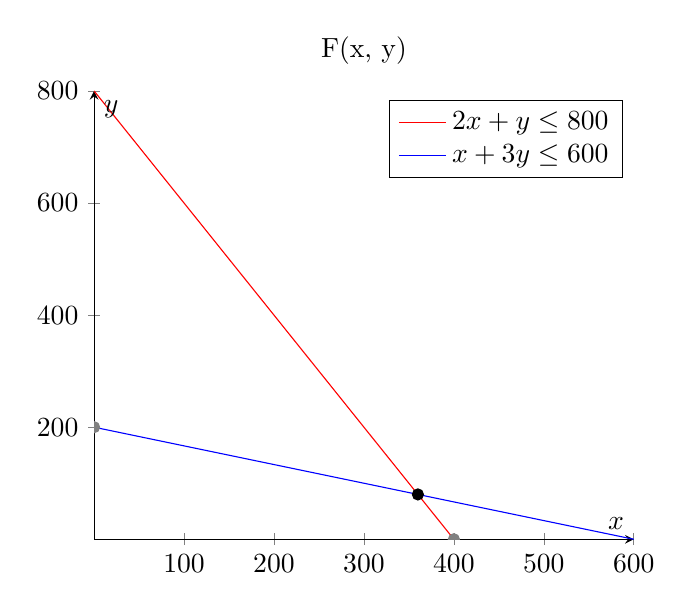
\begin{tikzpicture} 
                \begin{axis}[axis lines=middle,xlabel=$x$,ylabel=$y$,title={F(x, y)}]
                    
                    \addplot [
    domain=0:400, 
    samples=100, 
    color=red,
]
{800-2*x};
\addlegendentry{\(2x + y \leq 800\)}
%Here the blue parabola is defined
\addplot [
    domain=0:600, 
    samples=100, 
    color=blue,
    ]
    {(600-x)/3};
\addlegendentry{\(x + 3y \leq 600\)}
\filldraw[black] (360,80) circle (2pt);
\filldraw[gray] (0, 200) circle (2pt);
\filldraw[gray] (400, 0) circle (2pt);
                \end{axis}
            \end{tikzpicture} 
    \end{equation}
    \begin{equation}
        \begin{tabular}{|c | c | c|} 
            \hline
            x & y & F(x, y) \\
            \hline
            0 & 200 & 6000 \\ 
            \hline
            400 & 0 & 8000 \\
            \hline
            360 & 80 & 9600 \\
            \hline
           \end{tabular}
    \end{equation}
    \begin{equation}
        \begin{aligned}
            \text{Using the function } F(A, B) & = 20A + 30B \\
            F(x, y) & = 20x + 30y \\
            F(360, 80) & = 20(360) + 30(80) \\
            F(360, 80) & = 9600
        \end{aligned}
    \end{equation}
    \begin{equation}
        \text{The maximum of the function is at the point } (360, 80) 
    \end{equation}
    
\end{problem}